\subsection{Spatial Planning}
\label{subsec:spatial}

In enterprise wireless deployments, APs are usually scattered evenly across a building
to achieve good coverage, as in the case of our department building shown in
Figure~\ref{fig:floor}. However, there typically are certain public areas within
the building, such as lounges and conference rooms, where users tend to use the
wireless network more than other areas.

We first use the infrastructure side logs to study how the existence of public
areas affects the load distribution of the campus APs. We use three metrics to
quantify an AP's load during a period of time: number of \wifi{} sessions
served, total duration of \wifi{} sessions, and total traffic of all sessions.
For each of the 14 APs, we calculate these three load metrics during a 44 day
period from 03/12/2015 to 04/25/2015.

Figure~\ref{fig:load} shows the relative load distribution. We make several
observations. First, as expected, the load of APs near public areas, such as AP
3, 5, 4 and 12, are much higher than others. Second, interestingly, certain APs
near public areas, such as AP 7, are not as heavily loaded as other nearby APs.
Moreover, loads are not evenly distributed among APs that are near the same
public area, such as AP 3 and 5. Finally, we notice that the three load metrics
may produce inconsistent AP load ranks: some APs may serve fewer \wifi{}
sessions while still providing longer connection time or more traffic. In the
following discussion, we use session count as the load metric, since the other
two can be biased by factors such as applications or user behaviors.

From infrastructure logs, network operators can easily identify the hot spot APs
that are more heavily loaded than their neighbors. Two actions can then be taken
to deal with such load unbalance: \textit{redirection} and \textit{reposition}.
With \textit{redirection}, underutilized APs are left as is, so that
when nearby hot spot APs are congested, clients can be redirected to them for
load balancing. On the other hand, the underutilized APs can be
\textit{repositioned} to better locations to improve their utilization.

With only infrastructure measurements, however, it is not clear which approach
should be taken for each of the underutilized APs. Furthermore, in both
approaches, there are inherent challenges that are difficult to resolve.  When
redirecting the clients from a congested AP with a good signal to an idle AP with
a possibly worse signal, it is not clear what the impact on clients' network
performance will be. In addition, when there are multiple nearby underutilized APs as
offloading candidate, it is difficult to determine each AP's signal-load
tradeoff from clients' perspective. Finally when removing or repositioning
underutilized APs, it is challenging to predict how their load would
redistribute to nearby APs, or whether a coverage hole will be created.

In the rest of this section, we first show how smartphone measurements can be
used to build an empirical load balancing graph to help the network operator
make better load offloading decisions. Then we analyze how an AP's load would be
redistributed upon removal, to further help network operators evaluate the
impact of AP repositioning.


\subsubsection{Load Balance Graph}
\label{subsec:load_balance}

\begin{figure*}
  \centering
  \begin{minipage}[t]{0.31\textwidth}
    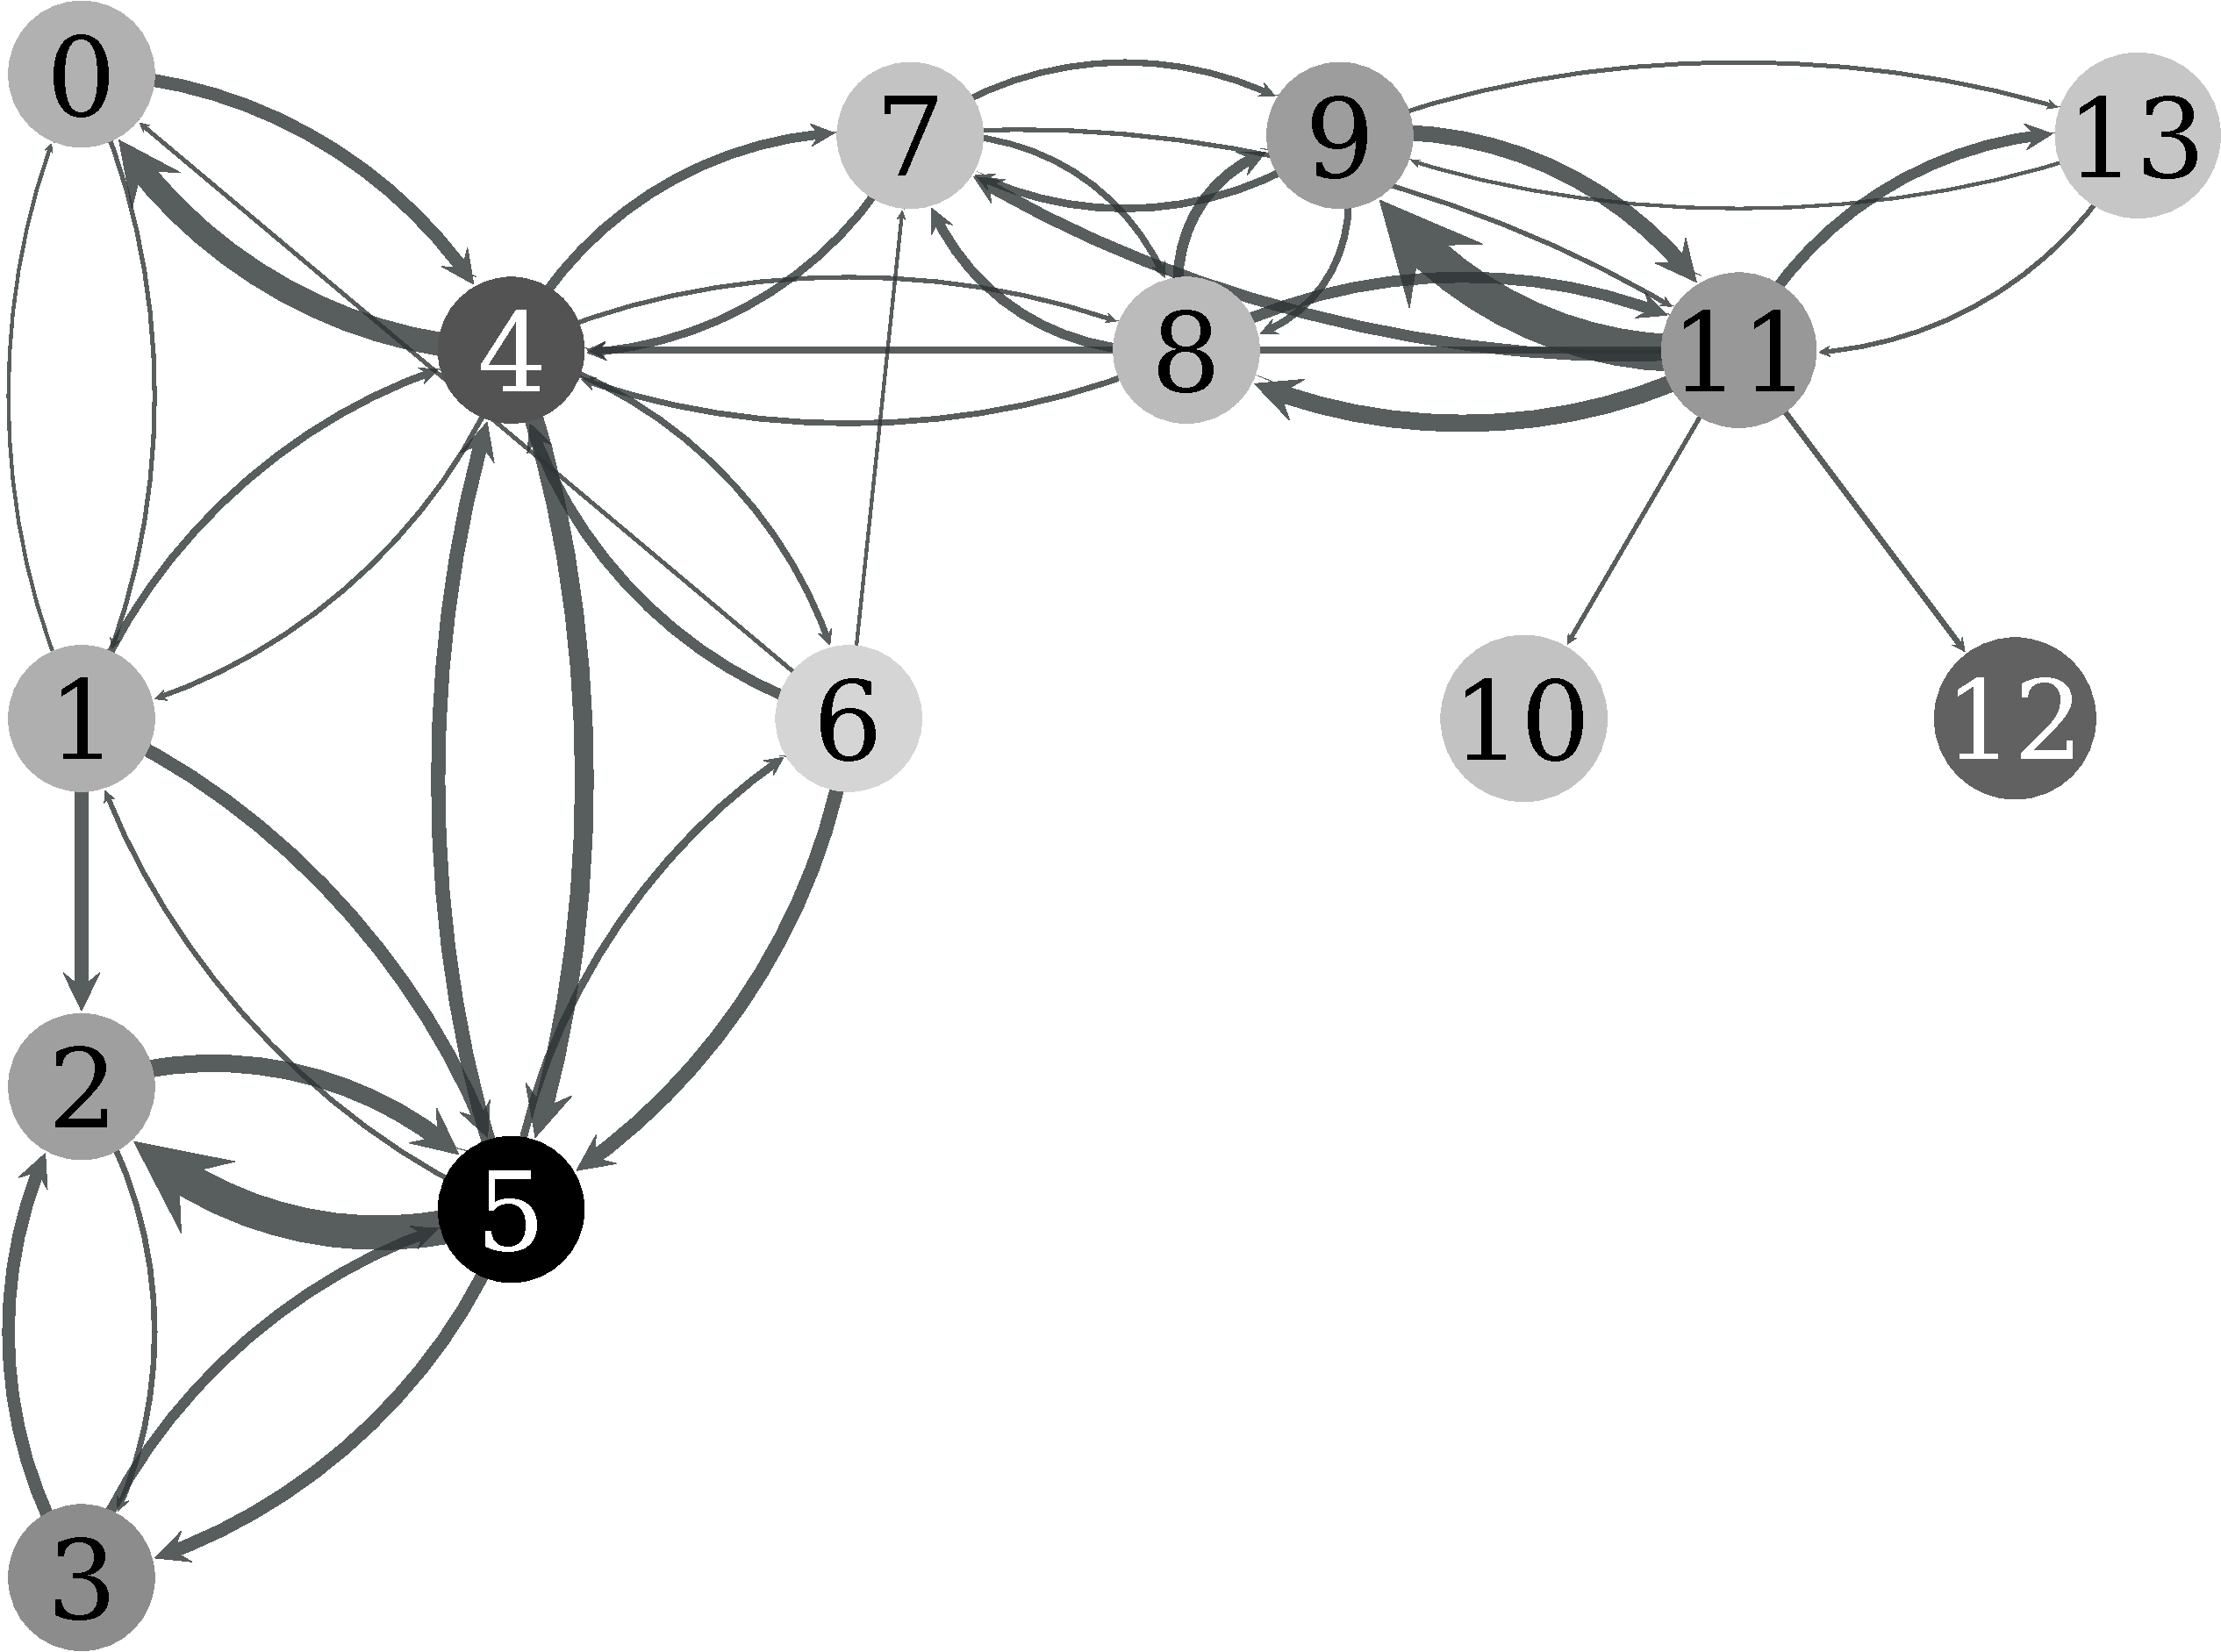
\includegraphics[width=\textwidth]{./figures/DavisLoadBalanceGraph.pdf}
    \caption{\textbf{Load Balance Graph.} Nodes are shaded based on 
      relative load. Edge width corresponds to $\langle device, timestamp \rangle$
    count in our dataset.}
    \label{fig:davis_load_balance}
  \end{minipage}\hspace{0.02\textwidth}%
  \begin{minipage}[t]{0.31\textwidth}
    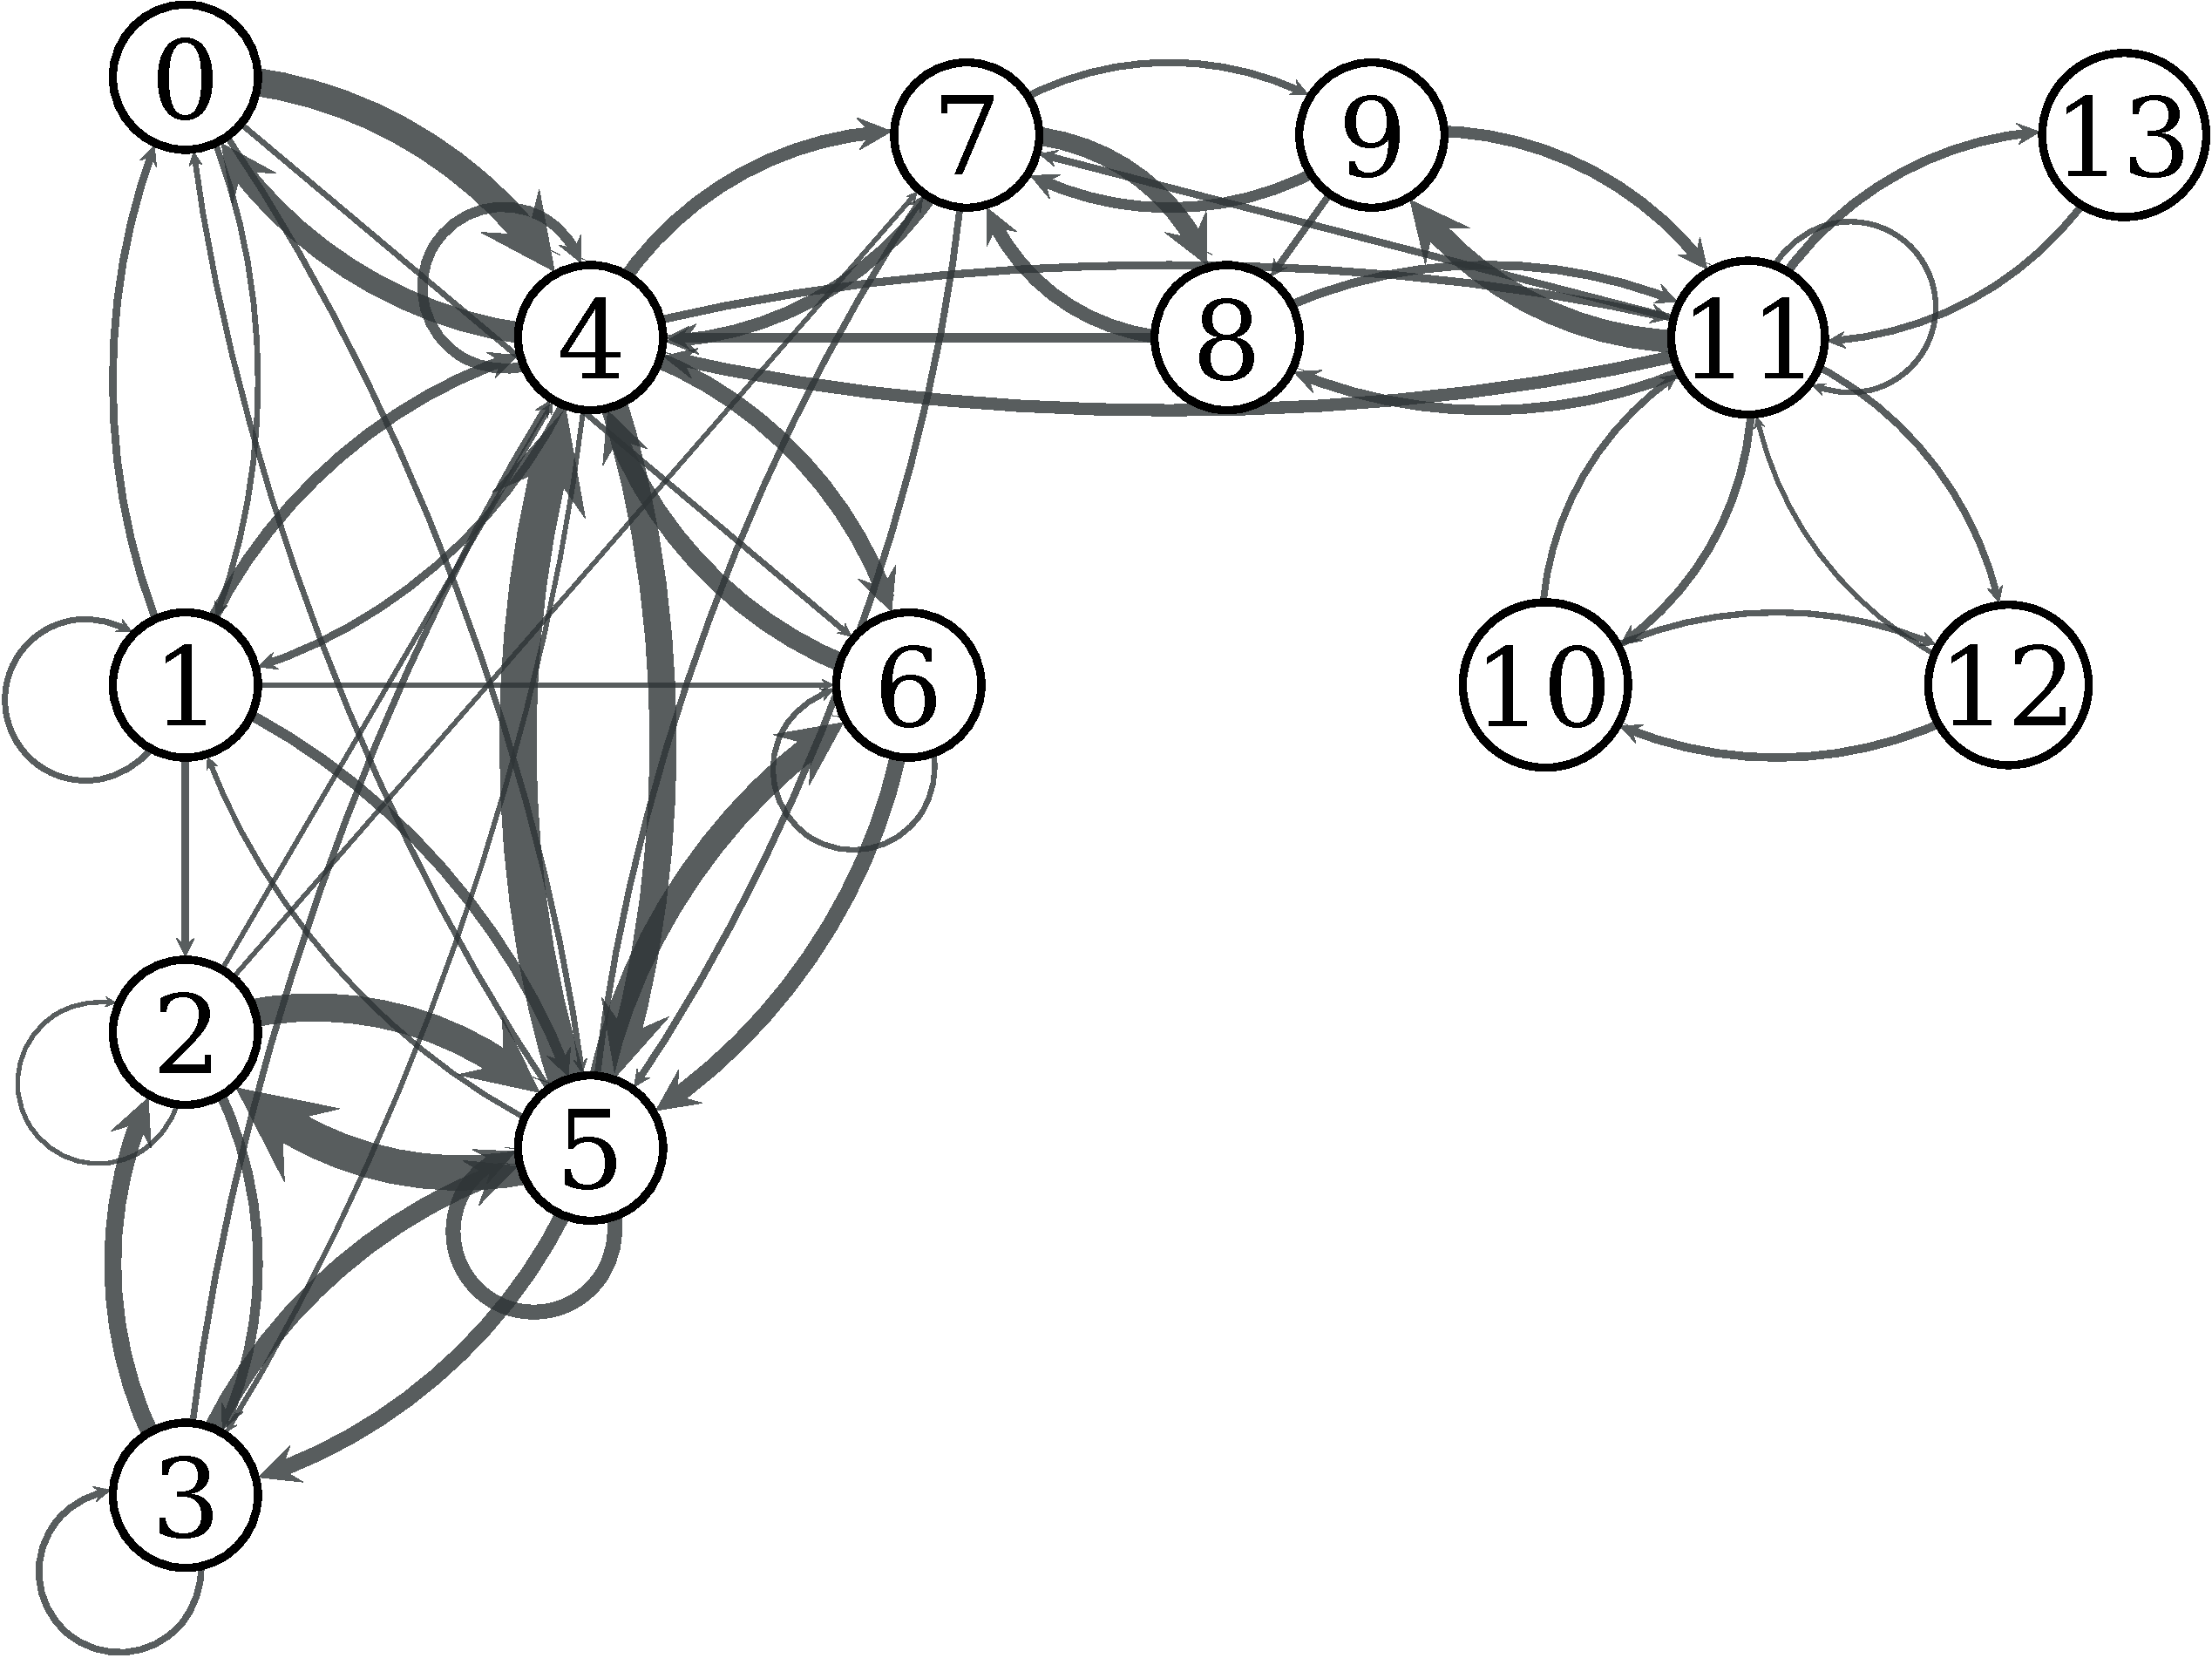
\includegraphics[width=\textwidth]{./figures/DavisLoadRedistributionGraph.pdf}
    \caption{\textbf{Load Redistribution Graph.} Edge width corresponds to the
    number of \wifi{} sessions shifted from the originating node.}
    \label{fig:davis_load_redist}
  \end{minipage}\hspace{0.02\textwidth}%
  \begin{minipage}[t]{0.31\textwidth}
    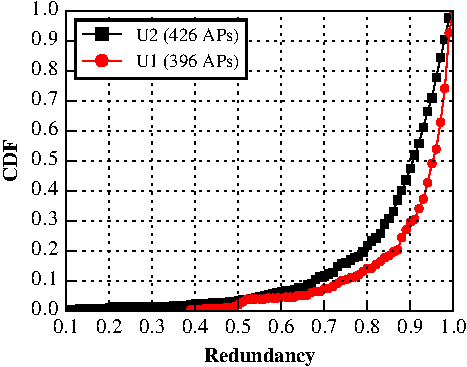
\includegraphics[width=\textwidth]{./figures/CampusAPRedundancyFigure.pdf}
    \caption{\textbf{CDF of Campus AP Redundancy.}}
    \label{fig:ap_redundancy}
  \end{minipage}
  \vspace*{\aftercaptiongap}
\end{figure*}

In enterprise wireless environment, where all APs use the same set of SSIDs and
authentication method, clients' association priority is solely based on each AP's
signal strength. However, it is well known that \wifi{} clients are usually
reluctant to roam to new APs unless the associated AP's signal strength
significantly drops below a certain threshold, which is as known as the ``sticky client''
problem. Therefore, the associated AP may not provide the best signal throughout
the entire \wifi{} session.

From load balancing perspective, it is useful to identify the subset of an AP's
neighbors which can potentially provide better signal to the AP's clients, such
that when the AP is overloaded, its clients can be redirected without
compromising their signal quality. With smartphone measurements, we can capture
such relationships using an \textit{empirical load balancing graph} $G_L = (V,
E_L)$, where $V$ is the set of APs, and $\langle AP_i \rightarrow AP_j \rangle
\in E_L$ if a client associated with $AP_i$ reports a better signal from $AP_j$
than $AP_i$. We also assign a weight to each edge to quantify how many times
such relationship is observed in the dataset.

Figure~\ref{fig:davis_load_balance} shows the $G_L$ constructed for the 14 APs
in the 3rd floor of our department building. Such a graph is useful in two ways. First, it
identifies backup APs for each hot spot AP for load balancing purposes. For
example, a large portion of AP 5 and 11's load can be shifted to AP 2 and 9
respectively without degrading client perceived signal quality. Second, it helps
to decide which action to take for each underutilized AP. For instance, edges
with large weight, such as $\langle 5 \rightarrow 2 \rangle$, $\langle 4
\rightarrow 0 \rangle$ and $\langle 11 \rightarrow 9 \rangle$, indicate that
those underutilized APs (2, 0 and 9) are better kept for load balancing
purposes. On the other hand, APs such as 7, 10 and 13 seldom provide better
signal than nearby hot spot APs, thus should be considered as reposition
candidates. However, even some of these candidate APs can not provide good
signal for load offloading purposes, they may exclusively serve certain users,
thus removing them will probably create coverage holes. We further look into
this in next section.


\subsubsection{Load Redistribution Graph}
\label{subsec:load_redist}

We now study how the load of a removed or broken AP would be
redistributed among its neighbor APs. This information is useful in two ways.
First, when repositioning underutilized APs, it is important to make sure that
the removal of the AP neither increases the burden of nearby hot spot APs
that are already heavily loaded, nor creates coverage holes for the clients that
were only able to connected to the removed APs. Second, when certain APs stop
accepting connections either temporally (e.g., due to scheduled maintenance) or
permanently (e.g., due to failure), network operators can use such information
to evaluate the impact of such unusual events on clients' network connectivity.

To this end, we can build a \textit{load redistribution graph} $G_R=(V, E_R)$ with
smartphone measurements as follows. Given the \wifi{}
scan result $R=(AP_1, AP_2,\ldots, AP_n)$ that is reported \textit{just before}
a \wifi{} connection with $AP_c \in R$, we remove $AP_c$ from $R$ and find the
AP with the best signal, denoted by $AP_s$. We draw an edge, $\langle AP_c
\rightarrow AP_s \rangle$, and increase its weight by 1. Intuitively, this
means if $AP_c$ is removed, the client's next \wifi{} session will be shifted to
$AP_s$. In a special case where $AP_c$ is the only AP in $R$, we draw a loop
edge $\langle AP_c \rightarrow AP_c \rangle$ and increase the edge weight by 1,
indicating that this next session would be lost if $AP_c$ is absent. To make
$R$ accurately reflect the device's network condition at the time of
association, we require that $R$ is reported no earlier than 10 seconds before the
connection event, and \wifi{} sessions without such scan results are not counted
towards $G_R$.

Figure~\ref{fig:davis_load_redist} shows the load redistribution graph for the
14 APs. Among the underutilized APs, AP 7 has medium 
incoming weights, indicating it is capable to provide backup connections
in case of neighbor AP failures. On other hand, AP 10 and 13 have very small incoming
weights, suggesting they may not be able to provide good signal for clients
that need to be redirected when neighbor APs fail. Additionally, there is no loop edges for
AP 10 and 13, meaning all the \wifi{} sessions they serve can be safely shifted to
nearby neighbor APs when they are removed. Therefore, AP 10 and 13 can be
repositioned to better places to increase their utilization. However, we must
note that the above conclusion is biased by the \wifi{} sessions of \PhoneLab{}
participants, thus may not be representative of all campus AP users. Further
investigations need to be conducted to reach a final decision.

We also observe from Figure~\ref{fig:davis_load_redist} that, for those heavily
loaded APs (e.g., AP 4 and 5), most of their loads can be shifted to nearby APs,
although certain number of connections will be dropped. To quantify this, we define an
AP's \textit{redundancy} as follows:

\begin{equation}
  \mathcal{R}(AP_i) = 1 - \frac{w_{AP_i \rightarrow AP_i}}{\sum_{j|AP_i \rightarrow
    AP_j \in E_R} w_{AP_i \rightarrow AP_j}}
\end{equation}

Where $E_R$ is the edges of redundancy graph, $w_{AP_i \rightarrow AP_j}$ is the weight (i.e., number of sessions)
of edge $\langle AP_i, AP_j\rangle$ in the load redistribution graph, and
$w_{AP_i \rightarrow AP_i}$ is the weight of $AP_i$'s loop edge. A large
redundancy means that most of $AP_i$'s connections can be safely shifted to its
neighbors.

We are now ready to analyze the redundancy of campus APs. To make the analysis
statistically meaningful, we only calculate the redundancy of APs whose total
outgoing weight is larger than a certain threshold (100). In total, we found
396 such APs from \ubscan{} dataset and 426 APs from \ndscan{} dataset.
Figure~\ref{fig:ap_redundancy} shows the CDF of these APs' redundancy. The
median redundancy is as high as 0.95 for \ub{} and 0.9 for \nd{} due to the dense AP
deployment within campus. We do notice, however, that about 5\% of the APs in
each campus are lower than 0.5. Such APs shall raise the attention of network
operators and may require further investigation for better spatial planning.


\subsubsection{Discussion}

We studied how to use the smartphone measurements to help the network operator
make load balancing decisions and evaluate the redundancy in AP spatial
planning. Note that the accuracy and usefulness of the two graphs largely depend
on the number of campus \wifi{} users who contribute measurements. In both
graphs, the edge weight and even the edge existence are biased by the subset of
users who report scan results. We discuss possible incentives to encourage
participation in data collection in Section~\ref{subsec:incentive}.

In addition, similar to the conflict graph discussed in
Section~\ref{subsec:channel}, the load balancing graph could potentially be built
in real time fusion. For instance, the congested AP could trigger a \textit{Frame
Report} on its clients and eagerly disassociate a client if it received better
signal from another campus AP. However, such real time coordination may further
add burden to the congested APs, thus a empirical graph built offline can still
be useful.
